\section{PRISM}\label{sec:method}
\subsection{Problem Formulation}\label{sec:formulation}
Given a time-series batch $\X\in\mathbb R^{B\times L\times C}$ with batch size $B$, window length $L$ and $C$ variables, let $\M\in\{0,1\}^{B\times L\times C}$ denote its observation mask. An entry $m_{n,t,c}=1$ indicates an observed value of variable $c$ at time $t$ in sample $n$; zero indicates a value to reconstruct. The input $\X_{\rm obs}$ retains visible values and sets unavailable entries to zero. Our objective is to reconstruct the complete window from these values and their mask:
\begin{equation}
 \widehat\X=\operatorname{PRISM}(\X_{\rm obs},\M).
 \label{eq:task}
\end{equation}

The output $\widehat\X\in\mathbb R^{B\times L\times C}$ preserves original measurements at observed entries and estimates missing entries.

As shown in Fig.~\ref{fig:architecture}, \Model{} combines Point-Level Context Encoding (PCE), Multi-Source Patch Evidence Construction (MPEC) and Pointwise Evidence-Guided Reconstruction (PEGR) to form an initial reconstruction $\X^{\rm i}$. Observation-Guided Residual Refinement (OGRR) then corrects this estimate using visible measurements. Point context describes current-window dynamics, patch evidence supplies local trends, and observation guidance further corrects reconstructed values.

\begin{figure*}[t]
 \centering
 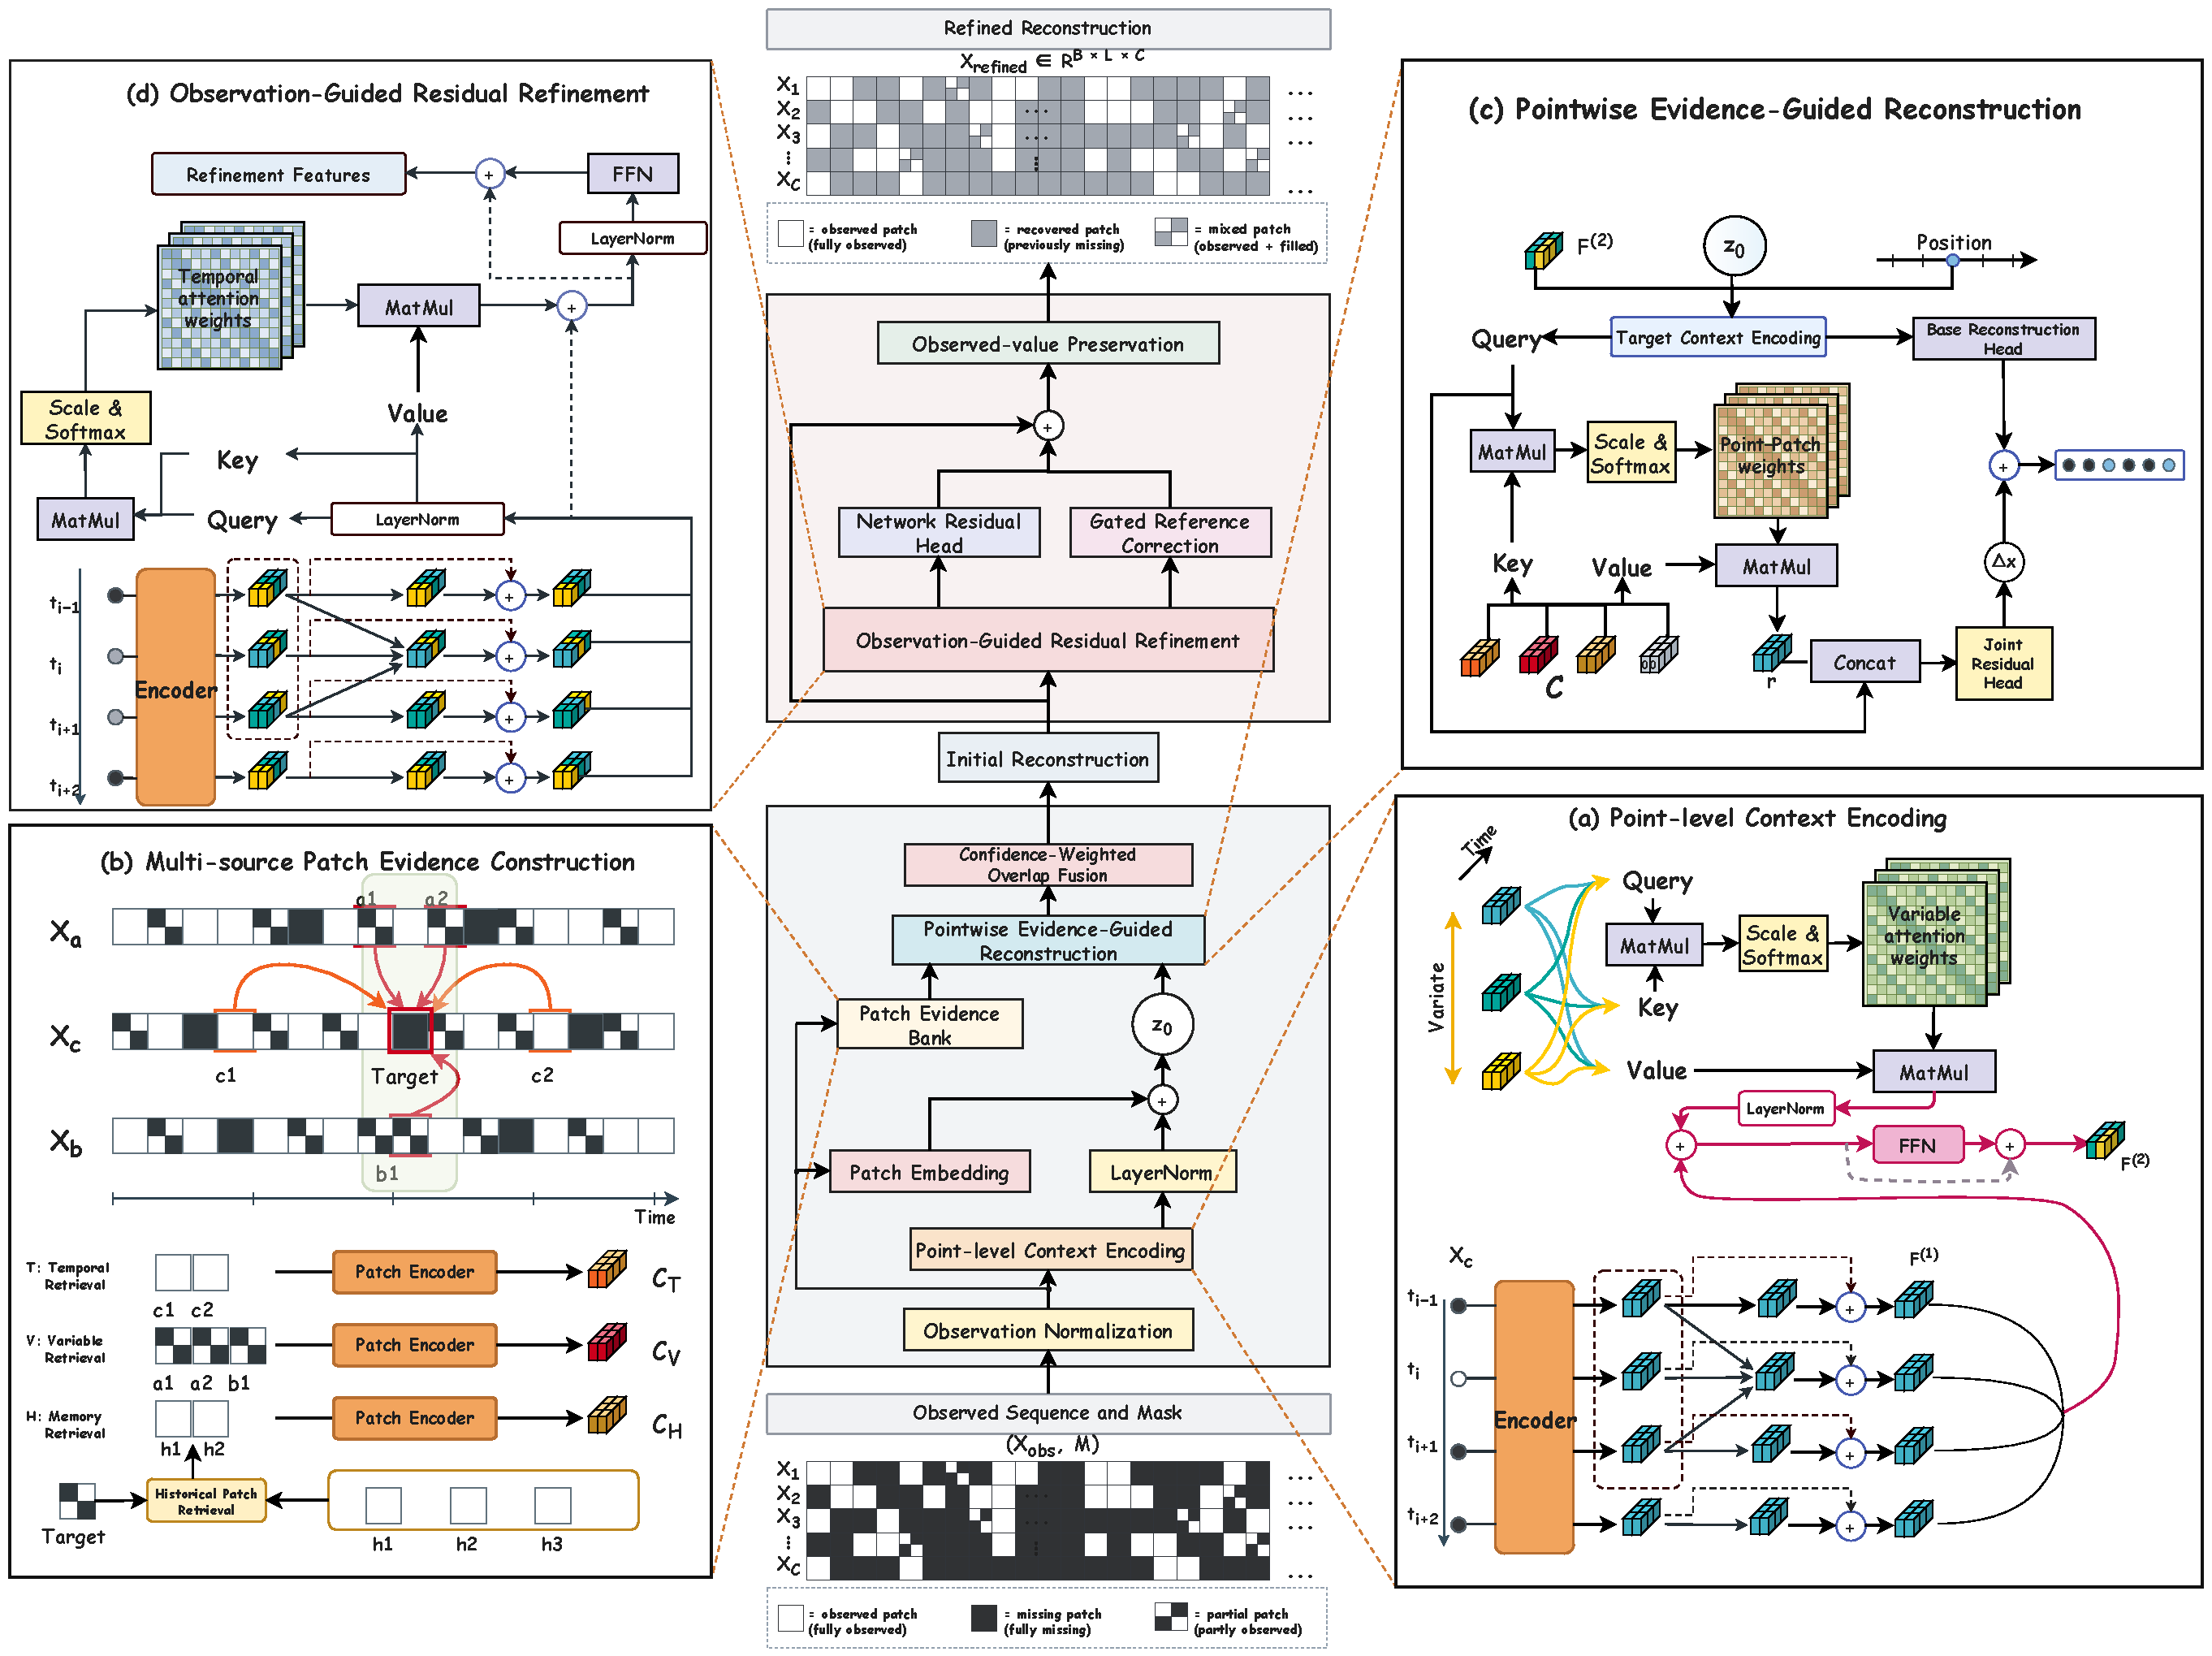
\includegraphics[width=\textwidth]{figures/prism_architecture.pdf}
 \caption{The framework of \Model. The observation-normalized input first passes through Point-Level Context Encoding (a), which combines residual temporal convolution and cross-variable attention. Multi-Source Patch Evidence Construction (b) organizes temporal, cross-variable and eligible training-history fragments into a common evidence bank. Pointwise Evidence-Guided Reconstruction (c) reads this bank with a target-specific query and jointly uses the query and readout to predict a residual over the base estimate. Confidence-weighted overlap fusion forms the initial reconstruction. Observation-Guided Residual Refinement (d) then combines this estimate with visible observations and mask information through residual temporal convolution and temporal attention. A neural residual head and a gated observation-reference correction jointly refine the missing values, while the final mask operation preserves observed measurements.}
 \label{fig:architecture}
\end{figure*}

\subsection{Point-Level Context Encoding}\label{sec:pce}
iTransformer organizes cross-variable interaction around variable trajectories~\citep{itransformer}, while T1 transfers temporal patterns through a temporal CNN and channel--head binding~\citep{t1}. Drawing on these ideas, PCE retains point-level temporal resolution and uses local dynamics together with variable relationships for both base reconstruction and subsequent patch-evidence reading. We call its temporal encoder Mask-Aware Temporal Convolution (MATC). Visible values, masks and visible-position relationships allow its updates to account for numerical variation and observation support. With input embedding $H$, encoding is
\begin{equation}
 \begin{split}
  \F&=\operatorname{VSAttn}\bigl(\operatorname{CNN}(\X_{\rm obs},\M)\bigr),\\
  z_{j,c}&=\phi_{\rm patch}([P^x_{j,c};P^m_{j,c}])
    +\psi\bigl(\operatorname{Pool}(\F_{\mathcal P_j,c})\bigr).
 \end{split}\label{eq:context}
\end{equation}

The tensor $\F^{(1)}$ represents temporal context and $\F^{(2)}$ represents integrated point context; both have dimensions $B\times L\times C\times d$. MATC produces temporal-convolution residuals; Temporal-Signature Variable Attention (TSVA) computes variable relationships from temporal feature signatures and produces cross-variable residuals that include feed-forward updates. Each feature channel supplies an attention pathway. Patch aggregation of this point context, combined with visible-value and mask embeddings, yields $z_0$, allowing point dynamics and local-fragment evidence to cooperate during reconstruction.

\subsection{Multi-Source Patch Evidence Construction}\label{sec:mpec}
PatchTST preserves local semantics through consecutive patches~\citep{patchtst}, while S4M supplements incomplete inputs with historical prototype representations~\citep{s4m}. MPEC retains individual fragments as point-queryable evidence and distinguishes temporal (T), cross-variable (V) and historical (H) sources. The target-patch index $i$ contains its sample, temporal position and variable; $c_i$ denotes its variable.

\paragraph{Temporal evidence T.}
Other patches of the same variable are organized into directional distance bands; each band scores and selects one fragment:
\begin{equation}
 \begin{aligned}
 s_{\rm T}(i,k)&=\begin{cases}
 -\operatorname{dist}(i,k),&k\in\mathcal B_{\rm near}(i),\\
 \langle\phi_{\rm T}(i),\psi_{\rm T}(k)\rangle/\sqrt d,&\text{otherwise},
 \end{cases}\\
 \mathcal C_{\rm T}(i)&=\left\{\operatorname{Top1}_{s_{\rm T}}(\mathcal B_{\rm T,d}(i))\right\}_{d\in\mathcal D},
 \end{aligned}\label{eq:temporal_selection}
\end{equation}

where $\mathcal B_{\rm near}(i)$ is the nearest band and $\operatorname{dist}$ measures patch distance. The mappings $\phi_{\rm T},\psi_{\rm T}$ project target and source features to dimension $d$. The set $\mathcal D$ contains nonempty bands, $\mathcal B_{\rm T,d}(i)$ retains eligible patches with visible support, and $\operatorname{Top1}$ selects the highest score. Near bands favor nearby structure; farther bands learn to match relevant dynamics.

\paragraph{Cross-variable evidence V.}
Variable relationships and current visibility jointly determine source scores and candidates:
\begin{equation}
 \begin{aligned}
 s_{\rm V}(i,v)&=a(c_i,v)+\tfrac12\rho(i,v)+\tfrac12\chi(i,v),\\
 \mathcal C_{\rm V}(i)&=\{x_{v,\delta}:v\in\mathcal S_{\rm V}(i),\ \delta\in\{-1,0,1\}\},
 \end{aligned}\label{eq:variable_selection}
\end{equation}

where $a$ is a learned variable relationship, $\rho$ measures visibility across neighboring source fragments, and $\chi$ measures consistency at commonly visible positions of aligned patches. The source variables are $\mathcal S_{\rm V}(i)=\operatorname{TopK}_{v\ne c_i}s_{\rm V}(i,v)$; $x_{v,\delta}$ is a patch from source $v$ at offset $\delta$ relative to the target. Only in-range fragments with visible support are retained.

\paragraph{Historical evidence H.}
Retrieval first locates an eligible same-variable historical group by key similarity, then scores and selects members within it:
\begin{equation}
 \begin{aligned}
 s_{\rm H}(i,h)&=\cos(e_i,e_h),\\
 \mathcal C_{\rm H}(i)&=\underset{x_h\in\mathcal A_{\rm H}(i)}{\operatorname{TopK}}s_{\rm H}(i,h),
 \end{aligned}\label{eq:history_selection}
\end{equation}

where $e_i,e_h$ are mask-aware target and member keys, and $\mathcal A_{\rm H}(i)$ contains patches satisfying temporal, provenance and similarity requirements in the selected group. Queries and members use consistent coordinates, and individual members retain local numerical structure. The bank is built exclusively from training data. Candidates from all three sources form $\mathcal C$, carrying source identities, quality, visible support and eligibility flags.

\subsection{Pointwise Evidence-Guided Reconstruction}\label{sec:pegr}
PEGR lets each target point read patch evidence independently through three steps: conditional projection, evidence residuals and base reconstruction.

\paragraph{Conditional projection.}
As shown in Fig.~\ref{fig:architecture}(c), $z_0$, point context $\F^{(2)}$ and position embedding $\mathbf P$ jointly construct the query, while the candidate bank $\mathcal C$ is projected to keys and values in parallel:
\begin{equation}
 q=\operatorname{Query}(z_0,\F^{(2)},\mathbf P),\quad [K,V]=\operatorname{KeyValue}(\mathcal C),
 \label{eq:point_qkv}
\end{equation}

where $z_0$ supplies the target patch's overall state, $\F^{(2)}$ retains temporal and variable context at the current point, and $\mathbf P$ distinguishes within-patch positions. The mapping $\operatorname{KeyValue}$ produces matching representations $K$ and readable content $V$ from the same candidate input.

\paragraph{Evidence reading and residuals.}
Point-to-Patch Evidence Attention (PPEA) reads the candidates, and the readout jointly determines the residual with the query:
\begin{equation}
 r=\operatorname{PPEA}(q,K,V),\quad \Delta x=\operatorname{MLP}(\operatorname{LN}([q;r])),
 \label{eq:point_residual}
\end{equation}

where PPEA computes scaled dot-product scores between $q$ and $K$, incorporates source priors, quality and eligibility, and uses Softmax-normalized weights to read $V$~\citep{attention}. The tensor $r$ is the readout. Concatenated features $[q;r]$ pass through layer normalization $\operatorname{LN}$ and the MLP's nonlinear mapping to generate $\Delta x$, together implementing the diagram's Joint Residual Head. Candidate corrections are zero when no candidate is eligible.

\paragraph{Base reconstruction and fusion.}
In parallel with evidence reading, the Base Decoder produces a contextual estimate. Adding the residual gives patch-level reconstruction:
\begin{equation}
 \X_{\rm base}=\operatorname{BaseDecoder}(z_0),\quad \X^{\rm c}=\X_{\rm base}+\Delta x,
 \label{eq:reconstruction}
\end{equation}

where $\X_{\rm base}$ is the base estimate and $\X^{\rm c}$ contains patch-level values corrected by evidence. Base decoding and residual outputs include their respective scale conversions, so both are added in the same coordinates. Overlapping patches are then assembled into a complete window:
\begin{equation}
 \X^{\rm i}=\operatorname{Fusion}(\X^{\rm c}),
 \label{eq:initial_fusion}
\end{equation}

where $\operatorname{Fusion}$ uses normalized confidence weights to combine patch estimates of the same position, excludes padding and preserves visible measurements. Thus $\X^{\rm c}$ becomes the complete initial reconstruction $\X^{\rm i}\in\mathbb R^{B\times L\times C}$ supplied to OGRR.

\subsection{Observation-Guided Residual Refinement}\label{sec:ogrr}
Initial reconstruction integrates point context and patch evidence, yet its numerical values can deviate in local level, variation amplitude or regions near visible boundaries. OGRR targets these deviations through residual correction. It combines temporal context in the reconstructed trajectory with numerical anchors from original visible measurements, forming the neural and gated-reference correction paths in Fig.~\ref{fig:architecture}(d).

\paragraph{Observation-conditioned features.}
The reference $\R$ is derived from visible neighbors of the same variable: linear interpolation with two-sided observations, or the available value with one-sided support. Support $U$ decays with observation distance and is zero when no reference exists. The discrepancy $D=U\Had(\R-\X^{\rm i})$ represents reference differences with observation support. We call this stage's local CNN Observation-Conditioned Temporal Convolution (OCTC). It jointly projects the initial estimate, visible values, mask, discrepancy and support, then extracts observation-conditioned features through local convolutional residuals:
\begin{equation}
 \mathbf H_{\rm ref}=\operatorname{TRA}\!\left(\operatorname{OCTC}([\X^{\rm i};\X_{\rm obs};\M;D;U])\right).
 \label{eq:refinement_features}
\end{equation}

The tensor $\mathbf H_{\rm ref}\in\mathbb R^{B\times L\times d_r}$ corresponds to Refinement Features in the diagram. OCTC extracts neighboring changes conditioned on observations; Temporal Refinement Attention (TRA) relates positions across the window. Its temporal-attention and feed-forward updates each include normalization and residual connections~\citep{attention}. Thus $\mathbf H_{\rm ref}$ describes the initial trajectory, observation locations and available reference discrepancies.

\paragraph{Neural residual correction.}
The Network Residual Head predicts corrections at missing entries, with corrections at visible entries set to zero:
\begin{equation}
 \Delta_{\rm net}=2\tanh\!\left(\operatorname{MLP}_{\rm net}(\mathbf H_{\rm ref})/2\right).
 \label{eq:neural_correction}
\end{equation}

The mapping $\operatorname{MLP}_{\rm net}$ projects the state to the variables, and the hyperbolic tangent bounds corrections to $[-2,2]$. This path learns reconstruction errors from temporal and cross-variable context without forcing corrections toward interpolation references. It is disabled for wholly unobserved windows.

\paragraph{Gated reference correction.}
The Gated Reference Correction adjusts reference discrepancies at missing entries with visible support, and is zero elsewhere:
\begin{equation}
 \Delta_{\rm ref}=G(\mathbf H_{\rm ref})\Had(\R-\X^{\rm i}).
 \label{eq:reference_correction}
\end{equation}

The gate $G$ is generated from $\mathbf H_{\rm ref}$ by a learned projection and hyperbolic tangent, taking values in $[-1,1]$. Positive gates follow the reference discrepancy, while negative gates allow reverse adjustments. The trajectory and observation support jointly determine the correction strength. This path is disabled when the variable has no visible reference. Encoding $U$ and $D$ allows the gate to account for reference distance and disagreement with the current estimate.

\paragraph{Observed-value preservation and output.}
Both corrections are added to the initial reconstruction to produce the final output:
\begin{equation}
 \widehat\X=\X^{\rm i}+\Delta_{\rm net}+\Delta_{\rm ref}.
 \label{eq:refinement}
\end{equation}

Corrections are zero at visible entries to preserve original measurements, corresponding to Observed-Value Preservation in the diagram. Both output heads are initialized to zero so OGRR learns corrections from the initial estimate. Its input interface also accepts initial results from other imputation backbones.

\subsection{Loss Functions}\label{sec:loss}
Let $\E$ denote the supervision mask. Initial reconstruction minimizes masked MSE with retrieval-key supervision and a numerical-level constraint; refinement minimizes weighted absolute error:
\begin{equation}
 \mathcal L_{\rm init}=\operatorname{MSE}_{\E}(\X^{\rm i},\X)+\lambda_k\mathcal L_{\rm key}+\lambda_l\mathcal L_{\rm level}.
 \label{eq:initial_objective}
\end{equation}
\begin{equation}
 \mathcal L_{\rm refine}=\frac{\|w\Had\E\Had(\widehat\X-\X)\|_1}{\|\E\|_1}.
 \label{eq:refinement_objective}
\end{equation}

The term $\mathcal L_{\rm key}$ combines retrieval-key alignment and contrastive supervision; $\mathcal L_{\rm level}$ constrains numerical levels. We set $\lambda_k=0.1$ and $\lambda_l=1$, and $w$ denotes the loss weights combining the implemented normalization rules. The initial reconstruction network, historical bank and retrieval encoders remain frozen during OGRR training.
